\documentclass[11pt,letterpaper]{article}
\PassOptionsToPackage{hyphens}{url}
\usepackage[margin=.83in,top=.8in,bottom=.8in,headheight=15pt]{geometry}
\usepackage[T1]{fontenc}
\usepackage{lmodern,amsmath,amssymb,mathtools,bm,booktabs,array,graphicx,tikz}
\usetikzlibrary{arrows.meta,positioning,calc,decorations.pathreplacing,patterns}
\definecolor{ink}{HTML}{17344D}\definecolor{accent}{HTML}{087E8B}\definecolor{pale}{HTML}{EDF5F5}\definecolor{gold}{HTML}{AD6B19}
\providecommand{\dd}{\,\mathrm{d}}\providecommand{\R}{\mathbb{R}}
\providecommand{\E}{\mathbb{E}}\providecommand{\Var}{\operatorname{Var}}
\providecommand{\Cov}{\operatorname{Cov}}\providecommand{\diag}{\operatorname{diag}}
\providecommand{\norm}[1]{\left\lVert#1\right\rVert}
\providecommand{\abs}[1]{\left|#1\right|}
\usepackage{microtype,hyperref,fancyhdr,enumitem,amsthm,sectsty,needspace}
\allsectionsfont{\raggedright}
\hypersetup{colorlinks=true,linkcolor=ink,urlcolor=accent,pdfauthor={Zan Ahmad},pdftitle={Population transfers: SIR dynamics, thresholds, and numerical conservation / Lecture notes}}
\setlength{\parindent}{0pt}\setlength{\parskip}{6pt}\linespread{1.07}
\setlist{itemsep=3pt,topsep=4pt,leftmargin=*}
\emergencystretch=2em\clubpenalty=10000\widowpenalty=10000
\pagestyle{fancy}\fancyhf{}\fancyhead[L]{\small Mathematical Modeling}\fancyhead[R]{\small Lecture 6}
\fancyfoot[L]{\footnotesize Zan Ahmad}\fancyfoot[R]{\footnotesize\thepage}\renewcommand{\headrulewidth}{.3pt}
\newtheorem{proposition}{Proposition}\newtheorem{theorem}{Theorem}\newtheorem{lemma}{Lemma}
\theoremstyle{definition}\newtheorem{definition}{Definition}\newtheorem{example}{Example}
\numberwithin{equation}{section}
\begin{document}
{\small\scshape Mathematical Modeling\hfill Lecture 6}\par\medskip
{\raggedright\hyphenpenalty=10000\exhyphenpenalty=10000\LARGE\bfseries\color{ink} Population transfers: SIR dynamics, thresholds, and numerical conservation\par}\medskip
{\small Lecture notes}\par\bigskip
A closed population changes composition through infection and recovery. From explicit contact assumptions we derive the SIR equations, establish their feasible state space, analyze their threshold and orbit, and construct a numerical update that respects the population budget.

\section{Population categories and contact assumptions}
\hypertarget{note-population-categories-and-contact-assumptions}{}\label{note:population-categories-and-contact-assumptions}
{\small \href{slides.html\#frame=a-closed-population-with-three-states\&step=1}{Slides for this section}}\par
Let $S(t)$, $I(t)$, and $R(t)$ denote susceptible, infectious, and recovered people. In this model recovery confers protection for the duration considered. The categories are disjoint and exhaust a closed population of size $N$: no births, deaths, migration, or return to susceptibility occur. We use continuous-valued group sizes as a deterministic population approximation. They need not be integers, and they are not claimed to be the exact expectations of an unspecified stochastic process.

Suppose a susceptible person makes potentially transmitting contacts at effective rate $\beta$, measured in $\mathrm{day}^{-1}$. Homogeneous mixing replaces the probability that the contacted person is infectious by $I/N$. The per-susceptible infection hazard is therefore $\beta I/N$, and the population transfer rate is
\[
J_{\mathrm{inf}}=\beta\frac{SI}{N}.
\]
A constant recovery hazard $\gamma$ gives $J_{\mathrm{rec}}=\gamma I$. Both fluxes have units of people per day. A constant hazard corresponds to an exponential residence-time model, not a common fixed infectious duration. The assumptions exclude latent stages, contact structure, and variation among individuals.
\begin{center}\begin{minipage}{.98\linewidth}\centering
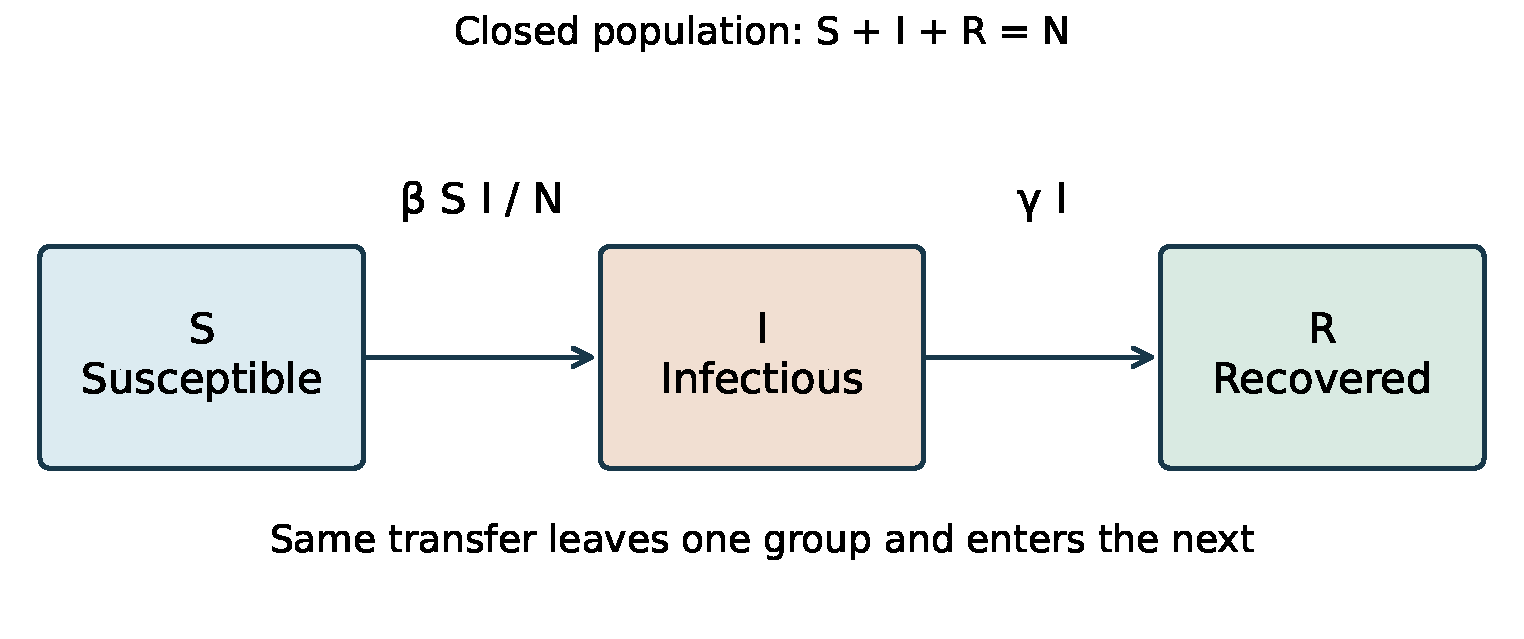
\includegraphics[width=.96\linewidth,height=.57\textheight,keepaspectratio]{population-transfers.pdf}\par\smallskip
{\small Original SIR schematic. Each transfer leaves one category and enters the next; recovered people remain inside the population and do not return to susceptibility in this model.}
\end{minipage}\end{center}
\section{Conservation, positivity, and the SIR equations}
\hypertarget{note-conservation-positivity-and-the-sir-equations}{}\label{note:conservation-positivity-and-the-sir-equations}
{\small \href{slides.html\#frame=derivation-of-the-sir-equations\&step=1}{Slides for this section}}\par
Infection transfers a person from $S$ to $I$; recovery transfers one from $I$ to $R$. Hence
\[
\boxed{\dot S=-\beta SI/N,\quad
\dot I=\beta SI/N-\gamma I,\quad
\dot R=\gamma I.}
\]
Adding the equations gives $\dot S+\dot I+\dot R=0$, so the initial total remains $N$. Conservation reduces the number of independent states to two, although storing all three is convenient for auditing the numerical budget.

The feasible set is the simplex $\{(S,I,R):S,I,R\geq0,\ S+I+R=N\}$. At $S=0$ or $I=0$, the corresponding outward transfer vanishes; at $R=0$, $\dot R=\gamma I\geq0$. More explicitly,
\[
S(t)=S_0\exp\!\left(-\frac\beta N\int_0^t I(s)\,\dd s\right),\qquad
I(t)=I_0\exp\!\left(\int_0^t[\beta S(s)/N-\gamma]\,\dd s\right).
\]
These expressions prove nonnegativity when the initial state is nonnegative. They also show that the deterministic model approaches an extinction limit continuously rather than removing the last infectious individual at a random time.
\section{Growth threshold and the infectious peak}
\hypertarget{note-growth-threshold-and-the-infectious-peak}{}\label{note:growth-threshold-and-the-infectious-peak}
{\small \href{slides.html\#frame=per-infectious-growth-rate\&step=1}{Slides for this section}}\par
For $I>0$, divide its equation by $I$:
\[
\frac{\dot I}{I}=\beta\frac SN-\gamma.
\]
When $\gamma>0$, define $\mathcal R_0=\beta/\gamma$ and the susceptible-dependent ratio $\mathcal R_{\mathrm{eff}}(t)=\mathcal R_0 S(t)/N$. Infectious prevalence grows when $\mathcal R_{\mathrm{eff}}>1$ and declines when it is below one. These are model parameters and a model threshold; no real intervention effect is estimated here.

For $N=1000$, $(S_0,I_0,R_0)=(990,10,0)$, $\beta=0.3\,\mathrm{day}^{-1}$, and $\gamma=0.1\,\mathrm{day}^{-1}$, the initial per-infectious growth rate is $0.297-0.1=0.197\,\mathrm{day}^{-1}$. Thus $\dot I(0)=1.97$ people per day. While $S$ remains close to $S_0$, $I(t)\simeq I_0e^{0.197t}$ is a local early-time approximation, not a full-outbreak solution.

Since $S$ decreases, the positive-infection trajectory reaches its interior peak when $S=N\gamma/\beta$, if it starts above that threshold. It need not exhaust susceptibility. With only $\beta$ changed to $0.08\,\mathrm{day}^{-1}$, the initial rate is $0.0792-0.1=-0.0208\,\mathrm{day}^{-1}$, and it cannot later turn positive because $S$ cannot increase.
\begin{center}\begin{minipage}{.98\linewidth}\centering
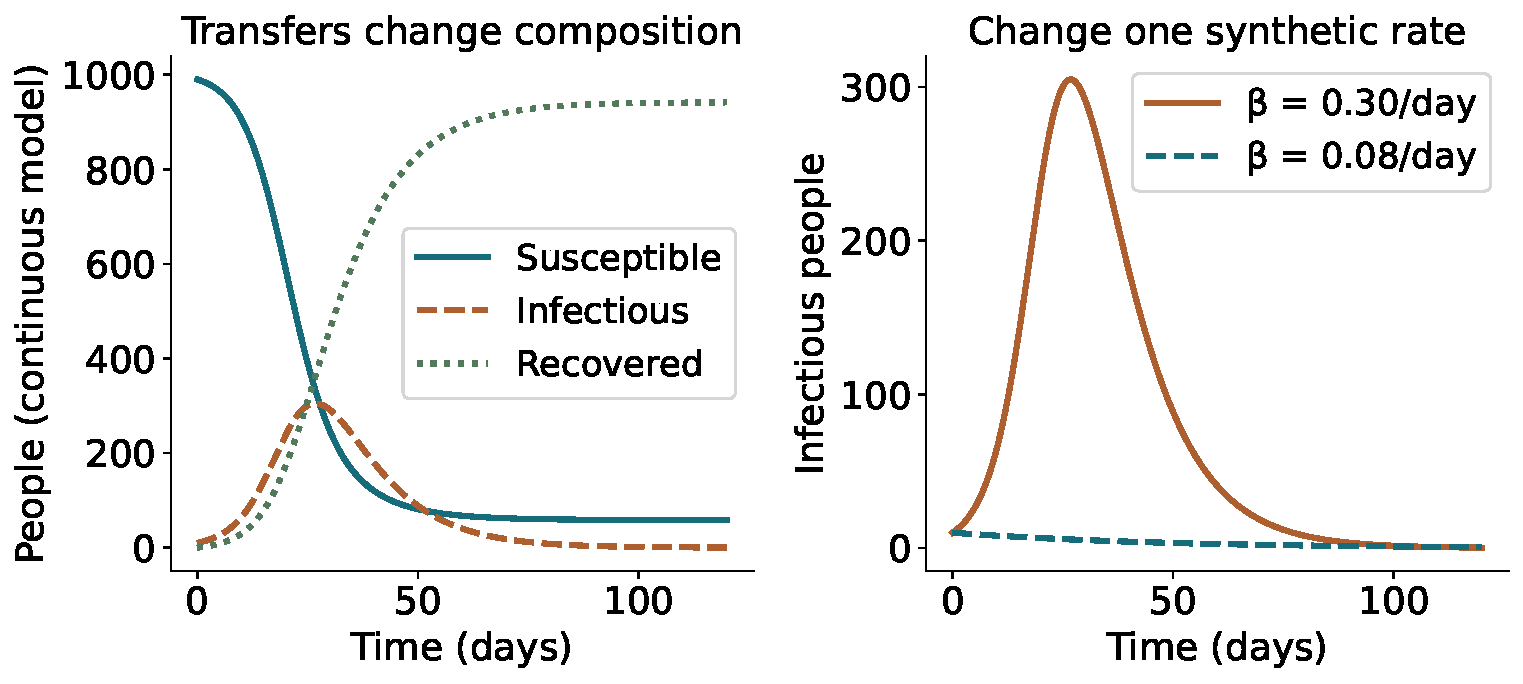
\includegraphics[width=.96\linewidth,height=.57\textheight,keepaspectratio]{population-trajectories.pdf}\par\smallskip
{\small Synthetic Euler trajectories at 0.1 day per step. Baseline N =\allowbreak{} 1000, initial (990, 10, 0), $\beta$ =\allowbreak{} 0.3/day and $\gamma$ =\allowbreak{} 0.1/day. The comparison changes only $\beta$ to 0.08/day.}
\end{minipage}\end{center}
\section{An invariant and the final-size relation}
\hypertarget{note-an-invariant-and-the-final-size-relation}{}\label{note:an-invariant-and-the-final-size-relation}
{\small \href{slides.html\#frame=eliminating-time-from-two-equations\&step=1}{Slides for this section}}\par
For constant positive $\beta,\gamma$, and while $S,I>0$, divide the infectious equation by the susceptible equation:
\[
\frac{\dd I}{\dd S}=-1+\frac{\gamma N}{\beta S}.
\]
Integration between the initial state and the current state gives a dimensionally meaningful logarithm,
\[
\boxed{I-I_0=-(S-S_0)+\frac{\gamma N}{\beta}\log\frac S{S_0}.}
\]
This relation describes the orbit in the $(S,I)$ plane without solving for time. It supplies an independent analytic comparison for a numerical trajectory; Euler preserves the population total exactly but generally does not preserve this nonlinear invariant exactly.

At an interior peak, substitute $S_p=N\gamma/\beta$ to obtain
\[
I_p=I_0+S_0-S_p+S_p\log(S_p/S_0).
\]
If $I(t)\to0$, the final susceptible count satisfies
\[
\log\frac{S_\infty}{S_0}
=-\frac\beta{\gamma N}(R_\infty-R_0),\qquad
R_\infty=N-S_\infty.
\]
This is an implicit equation, not a declaration that all susceptible people are eventually infected. The calculation is an analytical extension of the synthetic constant-parameter model. It does not turn its assumptions into empirical evidence.
\section{A conservative Euler step and its restrictions}
\hypertarget{note-a-conservative-euler-step-and-its-restrictions}{}\label{note:a-conservative-euler-step-and-its-restrictions}
{\small \href{slides.html\#frame=one-conservative-numerical-step\&step=1}{Slides for this section}}\par
Evaluate the two flows once at the start of an interval of length $h$ and reuse them with opposite signs:
\[
\begin{aligned}
S_{n+1}&=S_n-h\beta S_nI_n/N,\\
I_{n+1}&=I_n+h\beta S_nI_n/N-h\gamma I_n,\\
R_{n+1}&=R_n+h\gamma I_n.
\end{aligned}
\]
The sum is unchanged by exact arithmetic. For the stated initial state and a one-day step, infection transfers $2.97$ people and recovery transfers $1$ person. The updated state is $(987.03,11.97,1)$ and sums to $1000$.

The separate donor restrictions $h\beta I_n/N\leq1$ and $h\gamma\leq1$ ensure nonnegative updates. A sufficient uniform choice is
\[
h\max(\beta,\gamma)\leq1,
\]
because $I_n/N\leq1$. Indeed $S_{n+1}=S_n(1-h\beta I_n/N)$ and $I_{n+1}=I_n(1-h\gamma)+h\beta S_nI_n/N$ are then sums of nonnegative terms. This is an admissibility bound, not an accuracy estimate. The demonstration uses $h=0.1$ day and checks smaller steps. Two half-steps recompute the flows at the intermediate state, so they need not equal one full step.
\section{Numerical evidence and model discrepancy}
\hypertarget{note-numerical-evidence-and-model-discrepancy}{}\label{note:numerical-evidence-and-model-discrepancy}
{\small \href{slides.html\#frame=changing-one-transmission-parameter\&step=1}{Slides for this section}}\par
The original companion supplies two controlled scenarios, not a forecast fitted to observations. Check the population residual $S+I+R-N$, minimum group size, monotonic decrease of $S$, and monotonic increase of $R$. In the constant-parameter case, also compare the numerical $(S,I)$ trajectory with the orbit relation. Evaluate errors at common physical times when comparing time steps.

A curve can conserve $N$ exactly and still have an inaccurate peak height or peak time. Conversely, differences between observations and a converged solution may reflect omitted heterogeneity, observation processes, or changing parameters. Report the initial state, time unit, step, and the definition of the measured outcome before interpreting a comparison.

The reading introduces discrete epidemic models and their threshold reasoning. This companion uses a continuous-time SIR model with frequency-dependent incidence. Discrete infection probabilities and continuous hazards are related through a time interval; their numerical values must not be substituted for one another without conversion. A more detailed model requires a particular new mechanism and evidence, rather than additional compartments for their own sake.
\bigskip
\section*{Exercises}
\par\noindent\begin{minipage}{\linewidth}
\subsection*{MM06-E1. Transfer the same people twice}
Use N =\allowbreak{} 500, initial (S, I, R) =\allowbreak{} (480, 20, 0), $\beta$ =\allowbreak{} 0.25/day, $\gamma$ =\allowbreak{} 0.1/day and step h =\allowbreak{} 0.5 day.

\textbf{a} Compute the infection and recovery flows.

\end{minipage}\par\medskip
\textbf{b} Compute the two transfers and the next state.

\textbf{c} Check the total and explain the source of approximation.

\par\noindent\begin{minipage}{\linewidth}
\subsection*{MM06-E2. Predict growth without running a simulation}
Use $\beta$ =\allowbreak{} 0.3/day and $\gamma$ =\allowbreak{} 0.1/day with I > 0.

\textbf{a} Compare recruitment and recovery when S/N =\allowbreak{} 0.9. Does I initially grow?

\end{minipage}\par\medskip
\textbf{b} Repeat for S/N =\allowbreak{} 0.2.

\textbf{c} Find the susceptible fraction at balance and explain why I can decline before S reaches zero.

\par\noindent\begin{minipage}{\linewidth}
\subsection*{MM06-E3. Diagnose a smooth but wrong update}
At a step start, (S, I, R) =\allowbreak{} (900, 90, 10). The calculated infection transfer is 9 people and the recovery transfer is 18.

\textbf{a} Write the correct next state.

\end{minipage}\par\medskip
\textbf{b} A program instead returns (891, 82, 28). What invariant fails, by how much?

\textbf{c} Propose a repair and a separate accuracy check; explain why both are needed.

\par\noindent\begin{minipage}{\linewidth}
\subsection*{MM06-E4. State what a scenario establishes}
Two runs differ only in $\beta$. Both use synthetic parameters and the same closed-population assumptions.

\textbf{a} Name two limiting-case tests and their expected outcomes.

\end{minipage}\par\medskip
\textbf{b} Name an independent observation and an observation-process issue needed for real validation.

\textbf{c} Explain why a lower synthetic curve alone does not quantify the effect of a real intervention.

\section*{References}
\noindent\begin{minipage}{\linewidth}
Zan Ahmad, Fall 2024 HEART syllabus. PDF pages 1--2.

\end{minipage}\par\medskip
\noindent\begin{minipage}{\linewidth}
Hoppensteadt and Peskin, Modeling and Simulation in Medicine and the Life Sciences, second edition. Printed pages 300--304; PDF pages 311--315 in the supplied copy.

\end{minipage}\par\medskip
\end{document}
